\begin{frame}
 \frametitle{The Central Nervous System}
 \begin{columns}
\column{0.48\textwidth}
 \begin{itemize}
  \item All invertebrates except sponges and radially symmetric animals have one.
  \item Consist of spinal cord and brain in vertebrates.
  \item Tasked with gathering and processing information.
 \end{itemize}
  \column{0.48\textwidth}
  \begin{figure}[H]
  \centering
  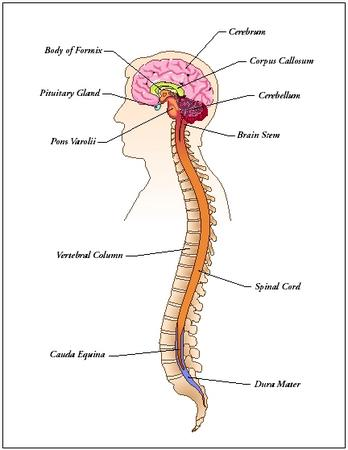
\includegraphics[scale=0.27]{figures/CNS.jpg}
  \caption{Human CNS}
  \end{figure}
 \end{columns}
\end{frame}



\begin{frame}
 \frametitle{Some words about the brain}
 \begin{columns}
\column{0.48\textwidth}
 \begin{itemize}
  \item Labeled the most complex object in the universe.
  \item $\sim200$ billion neurons with $\sim125$ trillion connections in neocortex alone.
  \item Different parts associated with different tasks.
  \item Many underlying processes are very inefficient.
 \end{itemize}
  \column{0.48\textwidth}
  \begin{figure}[H]
  \centering
  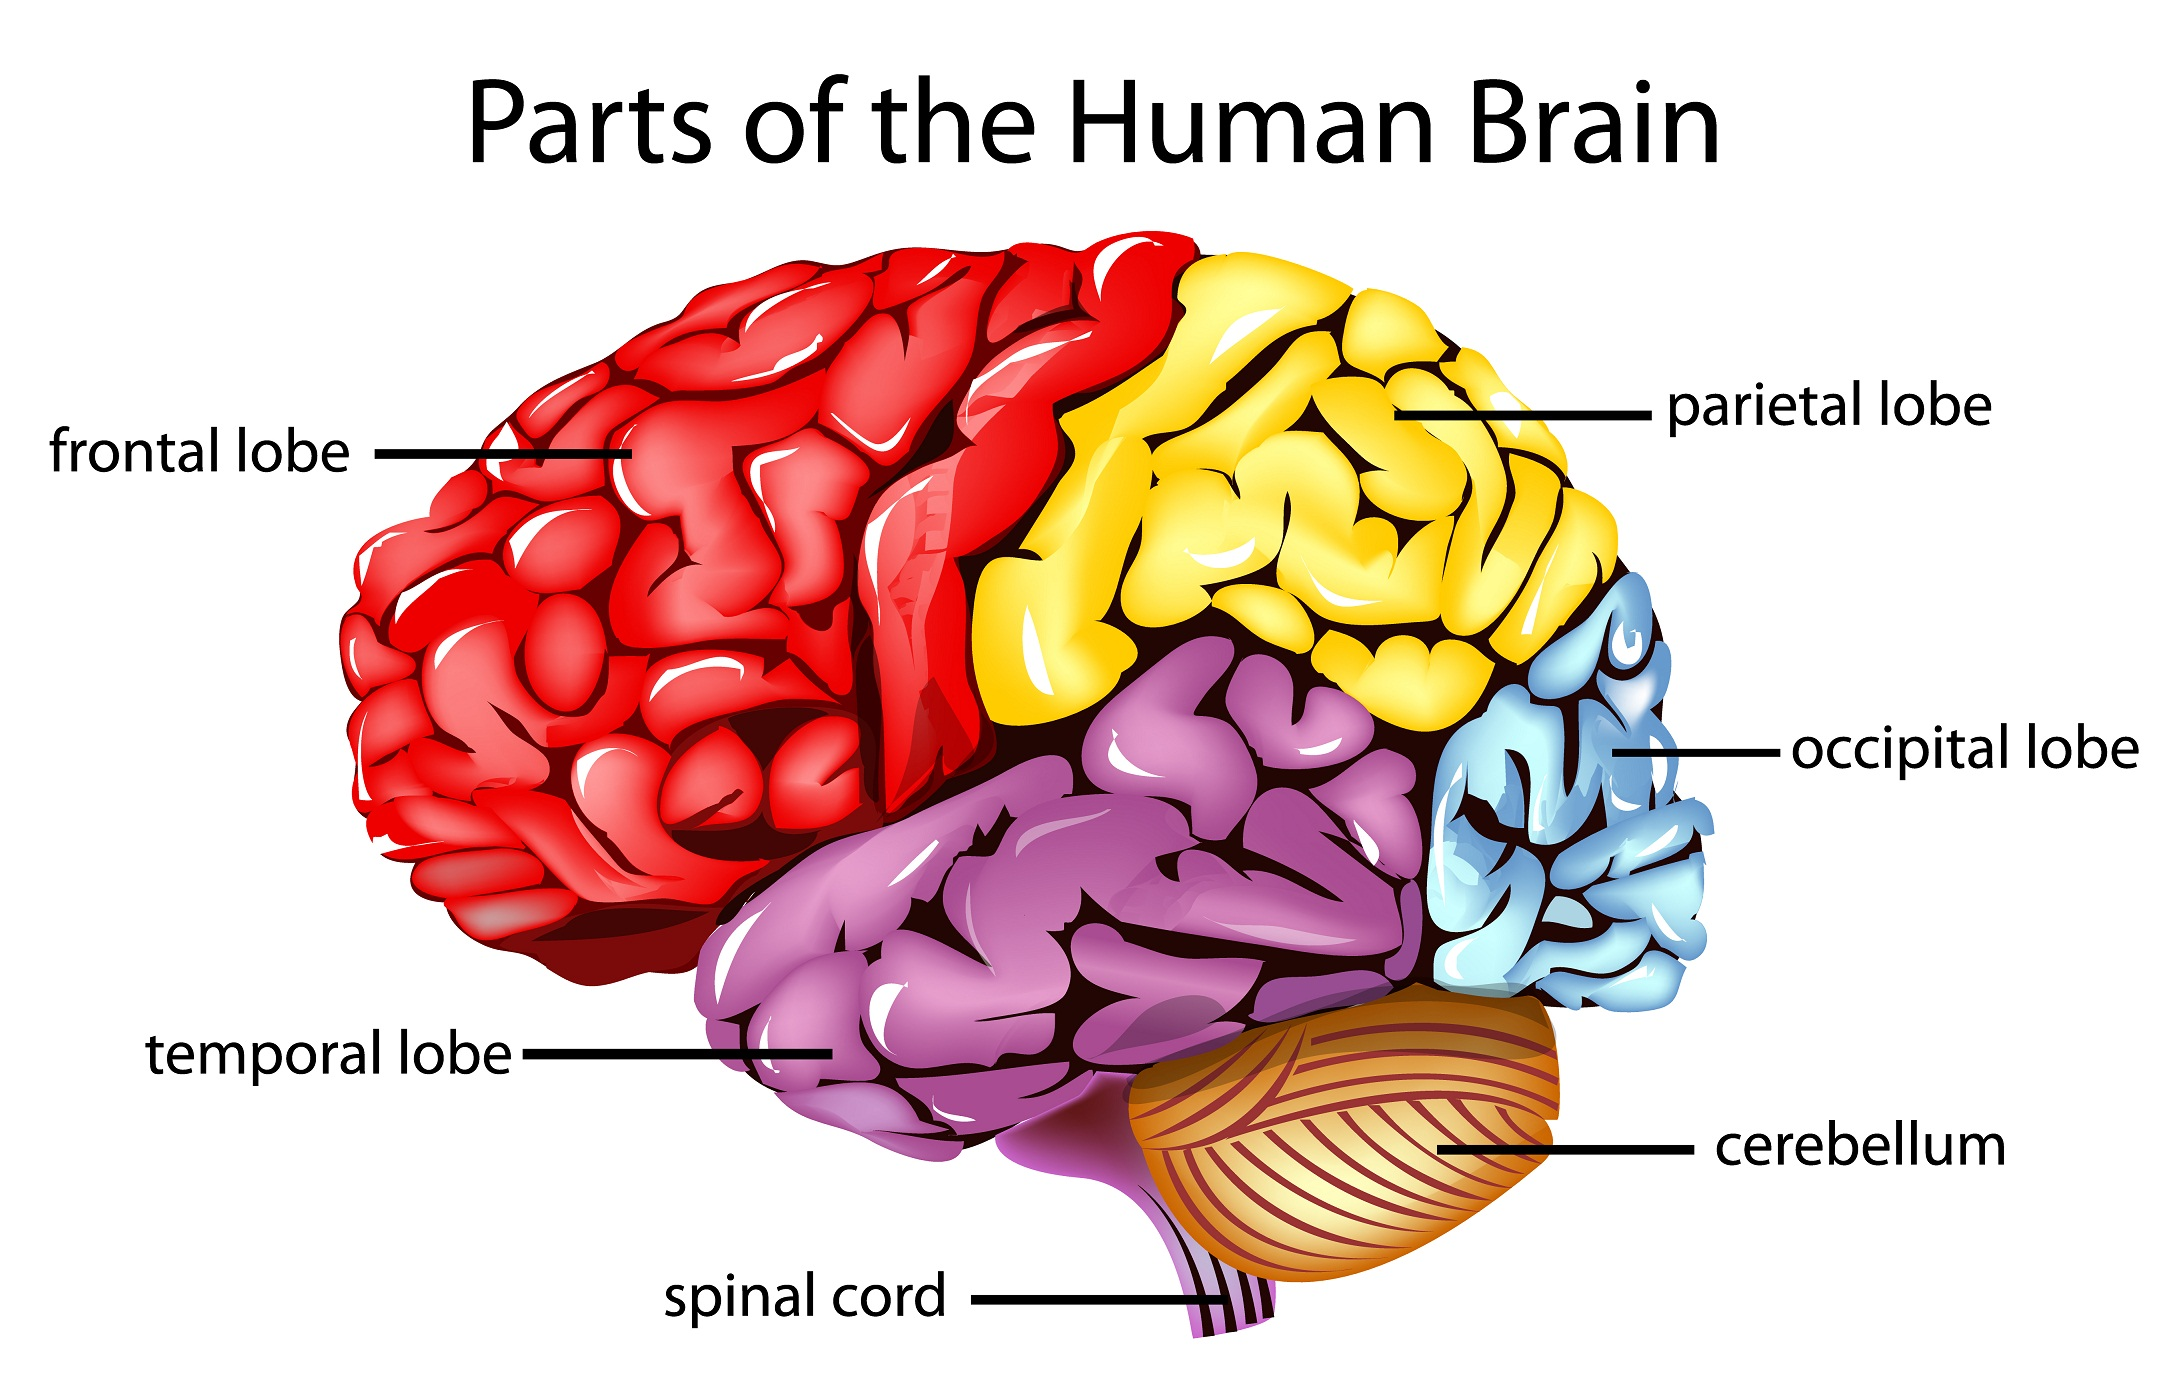
\includegraphics[scale=0.27]{figures/human_brain.jpg}
  \caption{Human brain with labels}
  \end{figure}
 \end{columns} 
\end{frame}


\begin{frame}
 \frametitle{Cells in the brain}
 \begin{columns}
\column{2.0in} Neurons:\\
\begin{itemize}
 \item Signal processing
\end{itemize}
\begin{figure}[H]
 \centering
 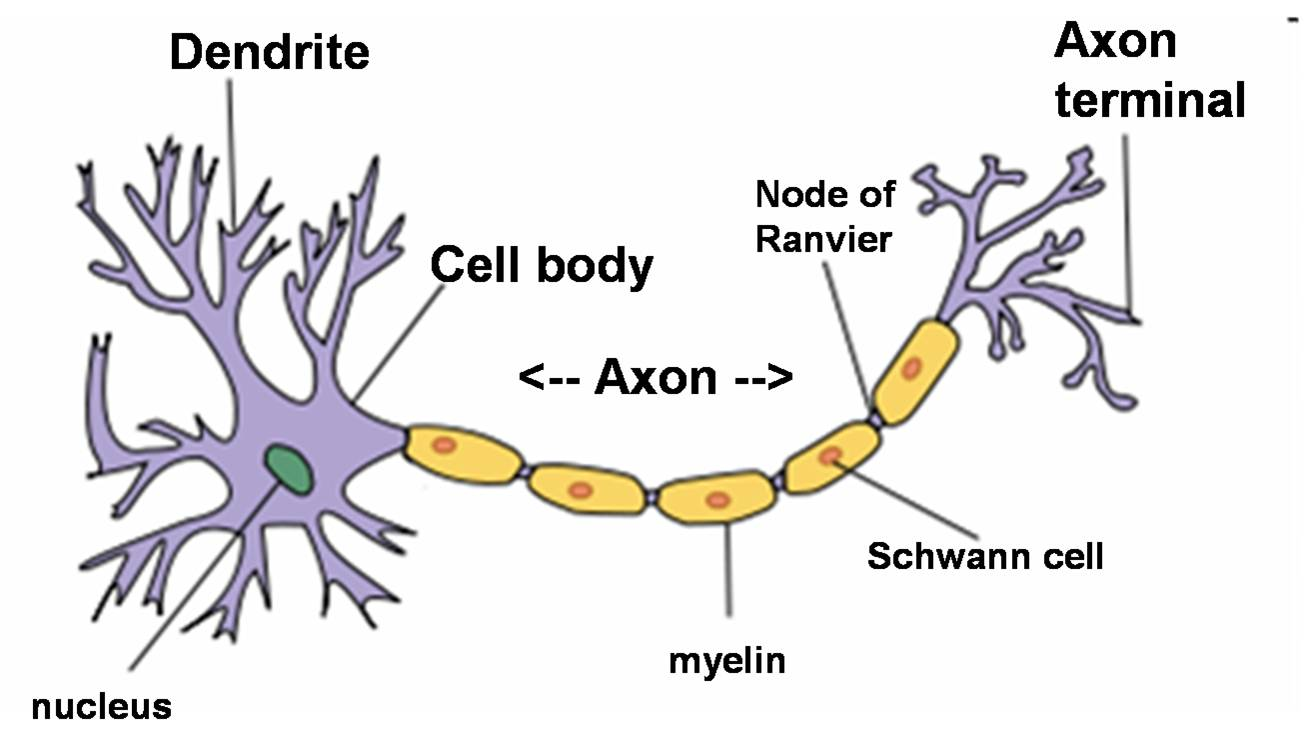
\includegraphics[width=\textwidth]{figures/neuron.jpg}
\end{figure}

\column{2.0in} Neuroglia:\\
\begin{itemize}
 \item Janitorial tasks
\end{itemize}
\begin{figure}[H]
 \centering
 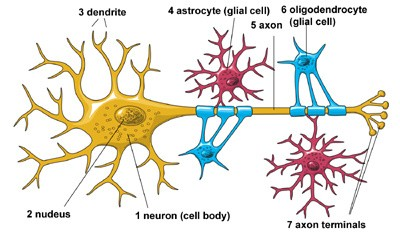
\includegraphics[width=\textwidth]{figures/neuroglia.jpg}
\end{figure}
 \end{columns}
\end{frame}
